\chapter{L'applicazione}
Durante il tirocinio è stata sviluppata un'applicazione scritta in Swift, con le seguenti funzionalità:
\begin{itemize}
\item La connessione ad un web server esterno inserendo username e password per accedere ad una libreria di dati multimediali
\item La visualizzazione delle immagini della libreria ed il salvataggio in una memoria cache, con tempo relativo alla singola sessione per una visualizzazione successiva
\item La riproduzione di file audio tramite il player di sistema, anche in background con lo schermo spento, e l'acceso ai controlli sulla schermata di blocco
\item La riproduzione di video della libreria tramite il player di sistema, anche in modalità Picture-in-Picture (PiP) se l'applicazione viene installata su iPad con il sistema operativo iOS 9.0 o successivi
\end{itemize}
\section{Implementazione}
L'applicazione è stata scritta in Swift 2.0 utilizzando XCode versione 7.0; per la parte web server è stato utilizzato un Raspberry Pi versione 1 con installato Debian 7 (denominato Wheezy) ed il server Apache 2.4. Per l'accesso ai dati dall'esterno è stato configurato sul server un client no-ip.\\\\
Sono stati inoltre utilizzati \textit{frameworks} esterni installati tramite il gestore di dipendenze CocoaPods ed una libreria scritta in Objective-C integrata tramite un \textit{bridging-header}.\\\\
Questi è un file .h che permette l'importazione di file interfaccia scritti in Objective-C per l'utilizzo in files scritti in linguaggio Swift, utilizzando la direttiva import del suddetto linguaggio.\\\\
L'interfaccia è stata implementata tramite un \textit{TabViewController}, contenente i tre \textit{UITableViewController} per le rispettive funzionalità denominate Immagini, Musica e Video.\\\\
Per la gestione della navigazione è stata utilizzata la modalità di \textit{segue} delle viste di iOS: fornendo un identificativo per la connessione tra un \textit{ViewController} ed un altro. Ciò permette, tramite la funzione \textit{prepare(for segue: UIStoryboardSegue, sender: Any?)} di intercettare l'instanziazione della nuova vista, e passare dati utili alla sua implementazione.\ 
\begin{figure}[H]
      \centering
      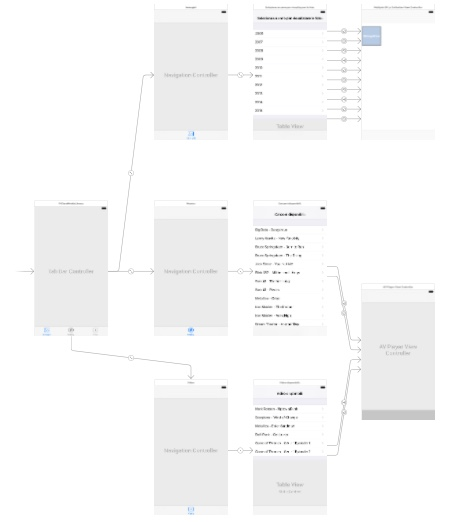
\includegraphics[scale=0.60]{immagini/app_views.jpg}
            \vspace{0.8cm}
            \caption{\textit{Le navigazioni dell'applicazione mostrate tramite \textit{Interface Builder}}}
\end{figure}
\newpage
\section{Schermate}
Di seguito verranno mostrate le schermate delle funzionalità.\\
\begin{figure}[H]
      \centering
      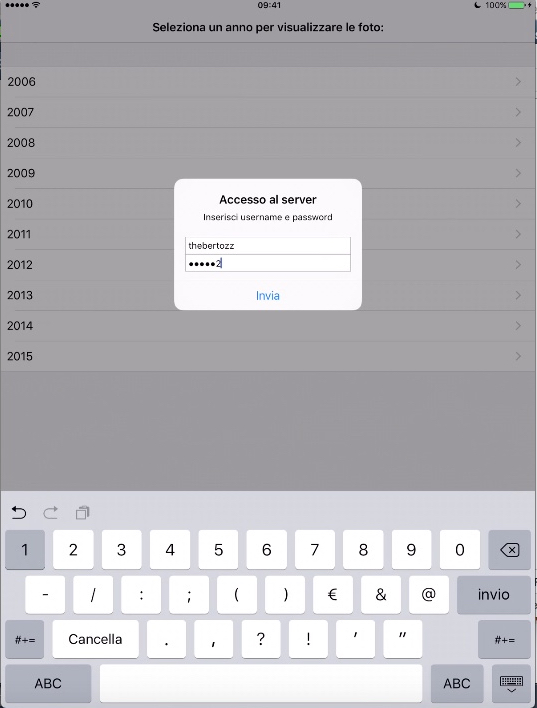
\includegraphics[scale=0.66]{immagini/app_login.jpg}
            \vspace{0.8cm}
            \caption{\textit{Fase di login al web server}}
\end{figure}
\begin{figure}[H]
      \centering
      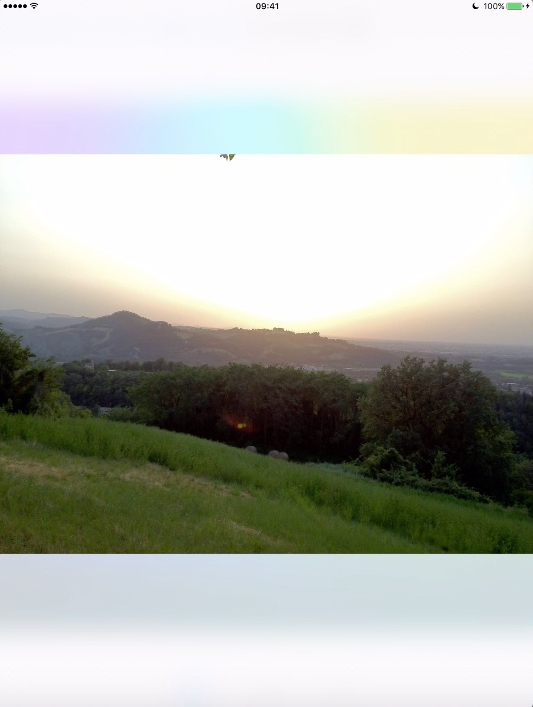
\includegraphics[scale=0.70]{immagini/app_foto.jpg}
            \vspace{0.8cm}
            \caption{\textit{L'applicazione può mostrare un array di immagini con zoom e pan e con scrorrimento orizzontale. Supporta lo swipe in qualunque direzione per tornare alla vista precedente}}
\end{figure}
\begin{figure}[H]
      \centering
      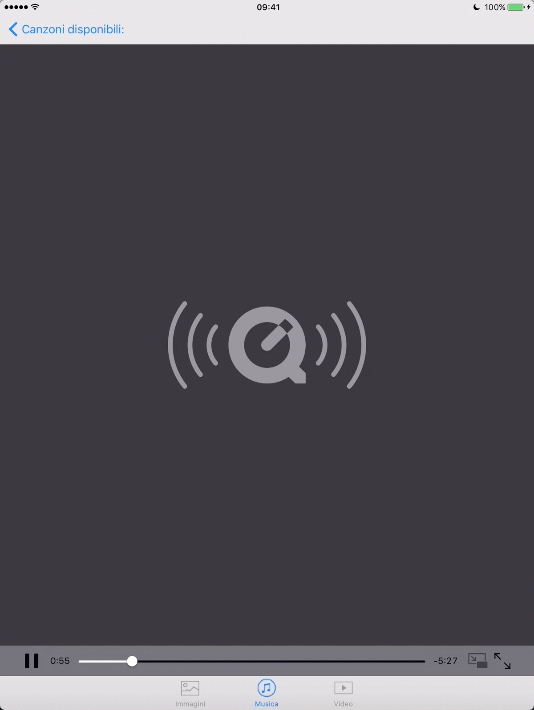
\includegraphics[scale=0.70]{immagini/app_audio.jpg}
            \vspace{0.8cm}
            \caption{\textit{La riproduzione audio, continua anche in background}}
\end{figure}
\begin{figure}[H]
      \centering
      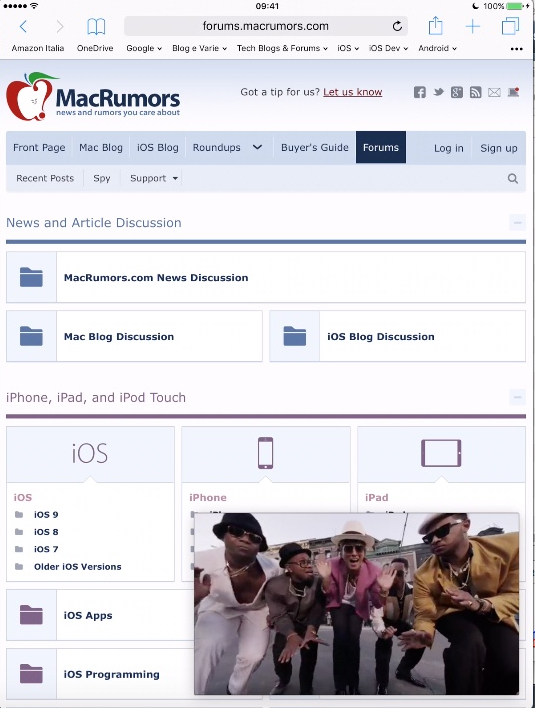
\includegraphics[scale=0.70]{immagini/app_video.jpg}
            \vspace{0.8cm}
            \caption{\textit{La modalità Picture-in-Picture per i contenuti video mostrata su iPad durante la navigazione web}}
\end{figure}
